\section{System Architecture}

\begin{table}[t]
\caption{Four Subsystems and Their Pi Interfaces}
\label{tab:interfaces}
\centering\footnotesize
\begin{tabularx}{\columnwidth}{@{}lX@{}}
\toprule
Subsystem & Connection and responsibility \\
\midrule
Vision / ML & CSI camera directly to Pi; local TFLite inference. \\
Navigation & LiDAR sensor controller and USB--UART path; ranging data consumed on Pi. \\
Wheel drive & USB serial, 9600 baud, to drive Arduino; PWM/direction through L298N. \\
Manipulator & Separate USB serial, 115200 baud, to arm Arduino; four servo channels. \\
\bottomrule
\end{tabularx}
\end{table}

\subsection{Central Computer and Physical Interfaces}
Figure~\ref{fig:architecture} shows the hardware interfaces; Fig.~\ref{fig:workflow} connects sensing and Pi processing to command generation through the reference coordinator. The analyzed configuration comprises a Pi Camera V2, YDLIDAR X4, L298N differential drive and servo arm; Table~\ref{tab:interfaces} lists the interfaces. A workstation supports visualization without hosting the native detector. Figures~\ref{fig:prototype} and~\ref{fig:front} show the prototype and laptop; the local display uses GPIO and the camera a white CSI ribbon. Figure~\ref{fig:dashboard} documents the command surfaces, not live-system performance.

\HazBotWorkflowFigure

% Original photograph with compact numbered markers; key stays in the caption.
\IfFileExists{figures/hazbot_prototype.pdf}{%
\begin{figure}[t]
\centering
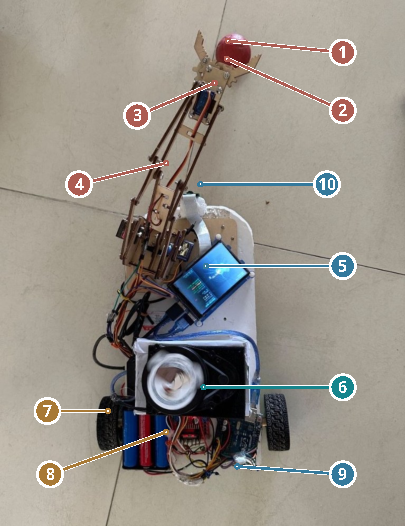
\includegraphics[width=0.78\columnwidth]{hazbot_prototype.pdf}
\caption{Physical HazBot prototype. Markers identify: 1, ball surrogate; 2, gripper; 3, servo; 4, arm linkage; 5, Raspberry Pi with GPIO-mounted display; 6, LiDAR; 7, drive wheel; 8, battery cells; 9, control electronics; 10, camera at the end of the white CSI ribbon.}
\label{fig:prototype}
\end{figure}
}{}

\IfFileExists{figures/hazbot_front.pdf}{%
\begin{figure}[t]
\centering
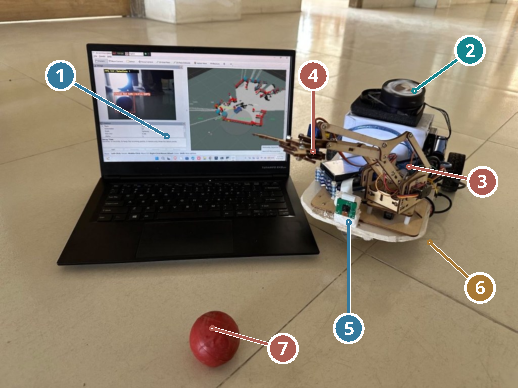
\includegraphics[width=\columnwidth]{hazbot_front.pdf}
\caption{Front view with laptop visualization. Markers identify: 1, laptop visualization; 2, LiDAR; 3, arm linkage; 4, gripper; 5, CSI camera; 6, mobile base; 7, ball surrogate.}
\label{fig:front}
\end{figure}
}{}


\subsection{Navigation and Wheel Control}
The LiDAR controller acquires ranges and sends packets to the Pi over USB. Host navigation uses scans for route clearance and target-distance association. ROS 2 mapping components are available, but map quality and localization error are not measured here.

The wheel Arduino drives the motor bridge independently of the arm controller. For an ideal differential base, wheel radius $R$ and track $b$ relate desired body velocity $(v,\omega)$ to wheel angular rates:
\begin{equation}
\dot\phi_L=\frac{v-b\omega/2}{R},\qquad
\dot\phi_R=\frac{v+b\omega/2}{R}.
\label{eq:drive}
\end{equation}
The model uses $R=0.033$\,m and $b=0.210$\,m. Realizing Eq.~\ref{eq:drive} requires a gateway that preserves wheel-rate semantics; the command study tests this condition.

\subsection{Vision and Native Inference}
The direct CSI path configures $640\times480$ RGB capture and a two-thread TFLite interpreter for an INT8 detector. Its tennis- and cricket-ball labels provide task surrogates. Hazard-related classes require a corresponding dataset and evaluation. Model weights are absent from the analyzed artifacts; accuracy and execution time are not reported.

A detection record should carry class, confidence, image position and age. Metric approach also requires range associated with the same target and frame. Class acceptance and freshness are distinct: a confident stale record cannot authorize approach. Task authority supplies handling permission; confidence establishes neither material identity nor authorization.

\subsection{Robotic Hand and Arm}
The arm has base yaw, shoulder pitch and elbow pitch, a fixed wrist and a separately actuated gripper. Its dedicated Arduino drives four servo channels, not four positioning joints. Existing commands include a preset pickup sequence; the seven-phase coordinator is a separate executable reference model. Separate drive and arm boards retain distinct serial protocols and pin assignments.
